\documentclass[problems]{esg8012pset} 
  \usepackage{amsmath}
  \usepackage{amssymb}
  \usepackage{enumerate}
  \usepackage{graphicx}
  \providecommand{\uvec}[1]{{\hat{\bf{#1}}}}
\classname{Physics 8.012} 
\semester{Fall 2010} 
\problemsetnumber{1} 
\date{September 8} 
\duedate{Friday, September 17} 
\readingassignment{Chapter One: Kleppner and Kolenkow, \emph {An Introduction to Mechanics}} 
\begin{document}
\section*{Problem 1: Fermi Problem (This problem is hard and should be a challenge.)}
  One of the moons of Jupiter, Europa, is reported to have its surface covered by an ocean of water
  which is 100 km deep.  The outermost 8 km are frozen as ice. The radius of Europa is
  approximately 1/4 the radius of the earth. Estimate the pressure at the bottom of Europa's ocean.
  (Note: there is some speculation that the combination of internal heat and water makes the ocean
  of Europa the best candidate in the solar system outside the earth for organized life to evolve.)
\section*{Problem 2: Kinematics-One Dimension}
  A bus leaves a stop at MIT and accelerates at a constant rate for 5 seconds. During this time the
  bus traveled 25 meters. Then the bus traveled at a constant speed for 15 seconds. Then the driver
  noticed a red light 18 meters ahead and slams on the brakes. Assume the bus decelerates at a
  constant rate and comes to a stop some time later just at the light.
  \begin{enumerate}[a)]
    \item What was the initial acceleration of the bus?
    \item What was the velocity at the bus after 5 seconds?
    \item What was the braking acceleration of the bus? Is it positive or negative?
    \item How long did the bus brake?
    \item What was the distance from the bus stop to the light?
    \item Make a graph of the position vs. time for the entire trip.
    \item Make a graph of the velocity vs. time for the entire trip.
    \item Make a graph of the acceleration vs. time for the entire trip.
  \end{enumerate}
\section*{Problem 3: Kinematics-One Dimension}
  You are a running as fast as you can at a constant velocity, $v_p$, trying to catch a bus that is at rest
  at a bus stop. When you are still a distance $b$ away from the bus stop, the bus starts to accelerate
  at a constant rate $a_\text{bus}$.
  \begin{enumerate}[a)]
    \item What is the minimum velocity that you need to run at in order to just catch the bus?
    \item Draw graphs showing the motion of the bus and yourself.
    \item How long did it take to catch the bus?
  \end{enumerate}
\section*{Problem 4: K\&K 1.7}
  Let $\uvec a$ and $\uvec b$ be unit vectors in the $xy$ plane making angles $\theta$ and $\phi$ with the $x$ axis,
  respectively. Show that $\uvec a = \cos\theta\uvec i + \sin\theta\uvec j$, $\uvec b = \cos\phi\uvec i + \sin\phi\uvec j$, and using vector algebra prove
that $\cos(\theta -\phi ) = \cos\theta \cos\phi + \sin\theta \sin\phi$.
\section*{Problem 5: K\&K 1.12}
  The acceleration of gravity can be measured by projecting a body upward and measuring the
  time that it takes to pass two given points in both directions. Show that if the time the body takes
  to pass a horizontal line $A$ in both directions is $T_A$ , and the time to go by a second line $B$ is $T_B$,
  then, assuming that the acceleration is constant, its magnitude is
  $$g = \frac{8h}{T_A^2 - T_B^2}$$
  \begin{center}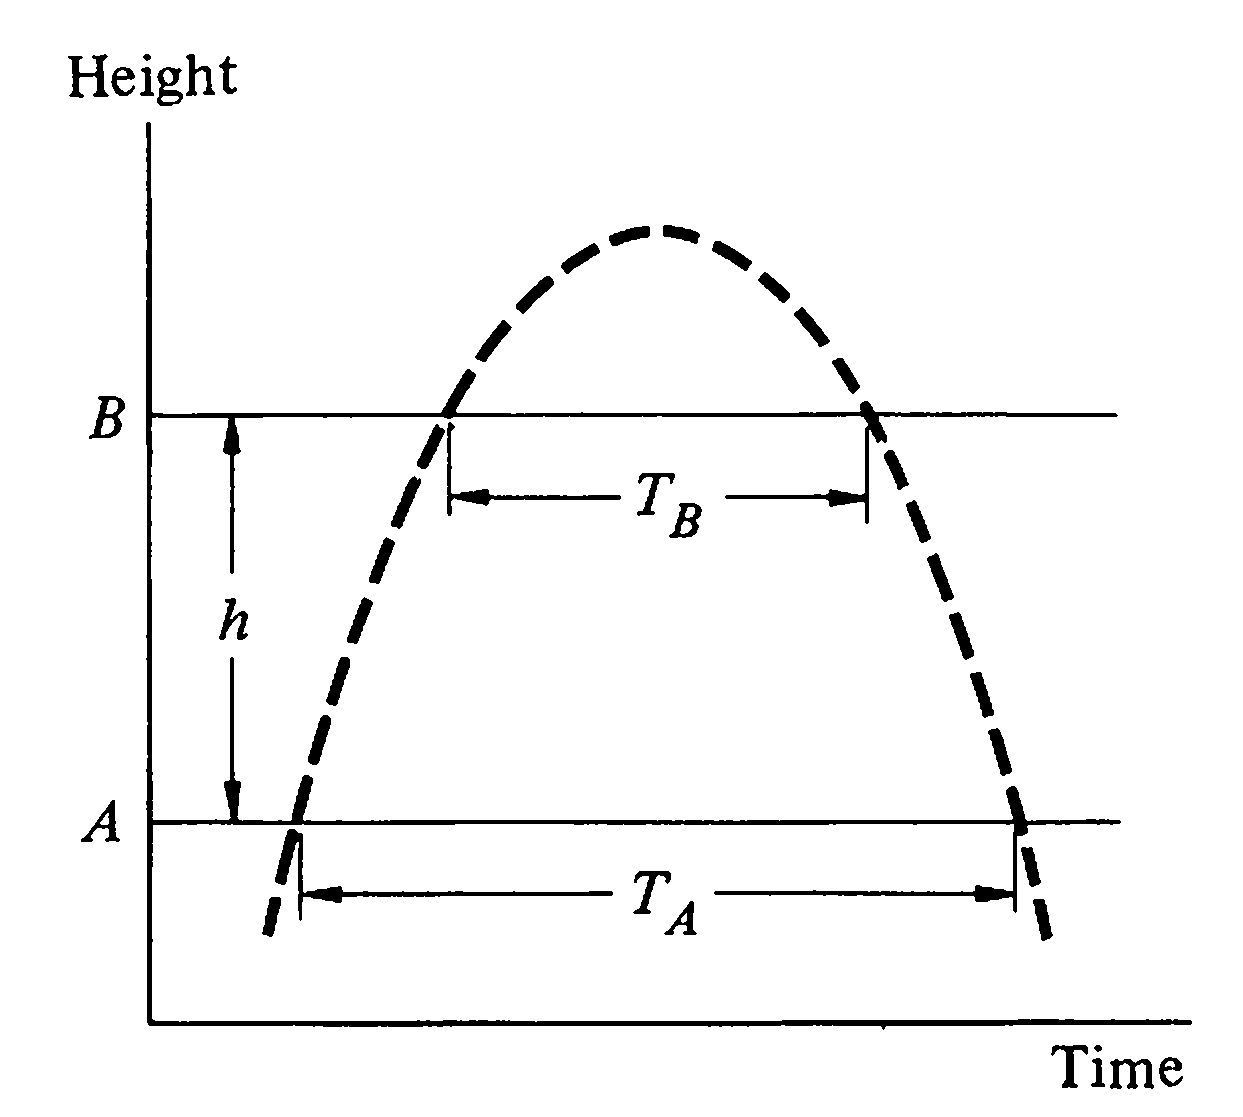
\includegraphics[width=0.35\textwidth]{ps01_1}\end{center}
